\begin{figure}
  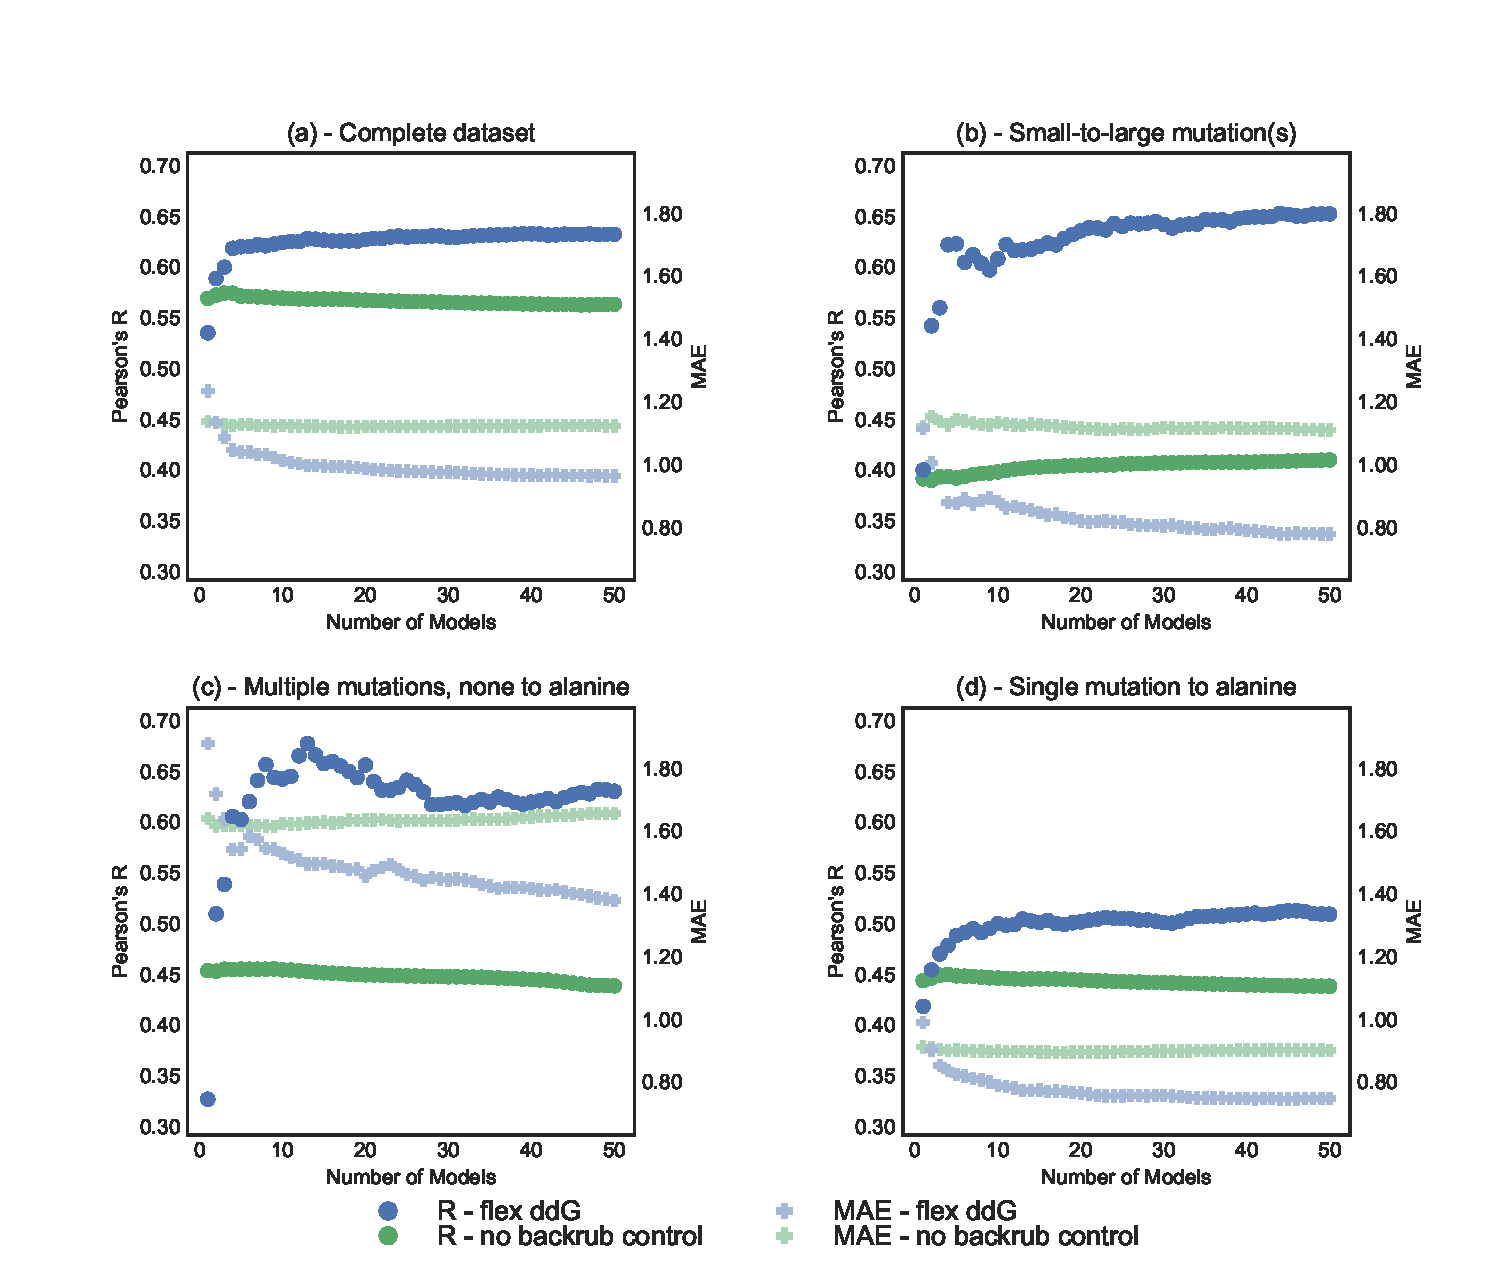
\includegraphics[width=\textwidth,keepaspectratio]{structs-v-corr-WildTypeComplex-zemu-12-60000-rscript-simplified-t14.pdf}
  \caption[]{
    Correlation (Pearson's R, left y-axis) and MAE (Mean Absolute Error, right y-axis) vs. number of averaged models (x-axis), on the complete ZEMu set, and subsets.
    Pearson's R is shown as circles, and MAE as faded plusses.
Predictions generated with the Flex ddG protocol are shown in blue.
Predictions generated with the no backrub control protocol are shown in green.
    A selection of key data underlying this figure can be found in \cref{tab:structs-v-corr-WildTypeComplex-zemu-12-60000-rscript-simplified-t14-underlying-data}.
    Structures are sorted by their minimized wild-type complex energy. 
    (a) Complete dataset (n = 1240, backrub steps = 35000)
    (b) Small-to-large mutation(s) (n = 130, backrub steps = 35000)
    (c) Multiple mutations, none to alanine (n = 45, backrub steps = 35000)
    (d) Single mutation to alanine (n = 748, backrub steps = 35000).
  } \label{fig:structs-v-corr-WildTypeComplex-zemu-12-60000-rscript-simplified-t14}
\end{figure}
